\section{Comparación}

Para poder ilustar mejor las diferencias entre las imágenes originales y las comprimidas, tanto en escala de grises como en color, se creó un notebook de Jupyter que presenta los resultados visuales. Esta notebook fue generada con apoyo de herramientas con inteligencia artificial y cumple únicamente el proposito de demostración gráfico y no afecta directamente en el desarrollo técnico de proyecto.

\subsection{Imagenes de comparación}

\begin{figure}[htbp]
  \centering
  \includegraphics[width=0.8\textwidth]{sources/comparison/test_1.png}
  \caption{Resultados de compresión imagen 1}\label{fig:comparison1}
\end{figure}

\begin{figure}[htbp]
  \centering
  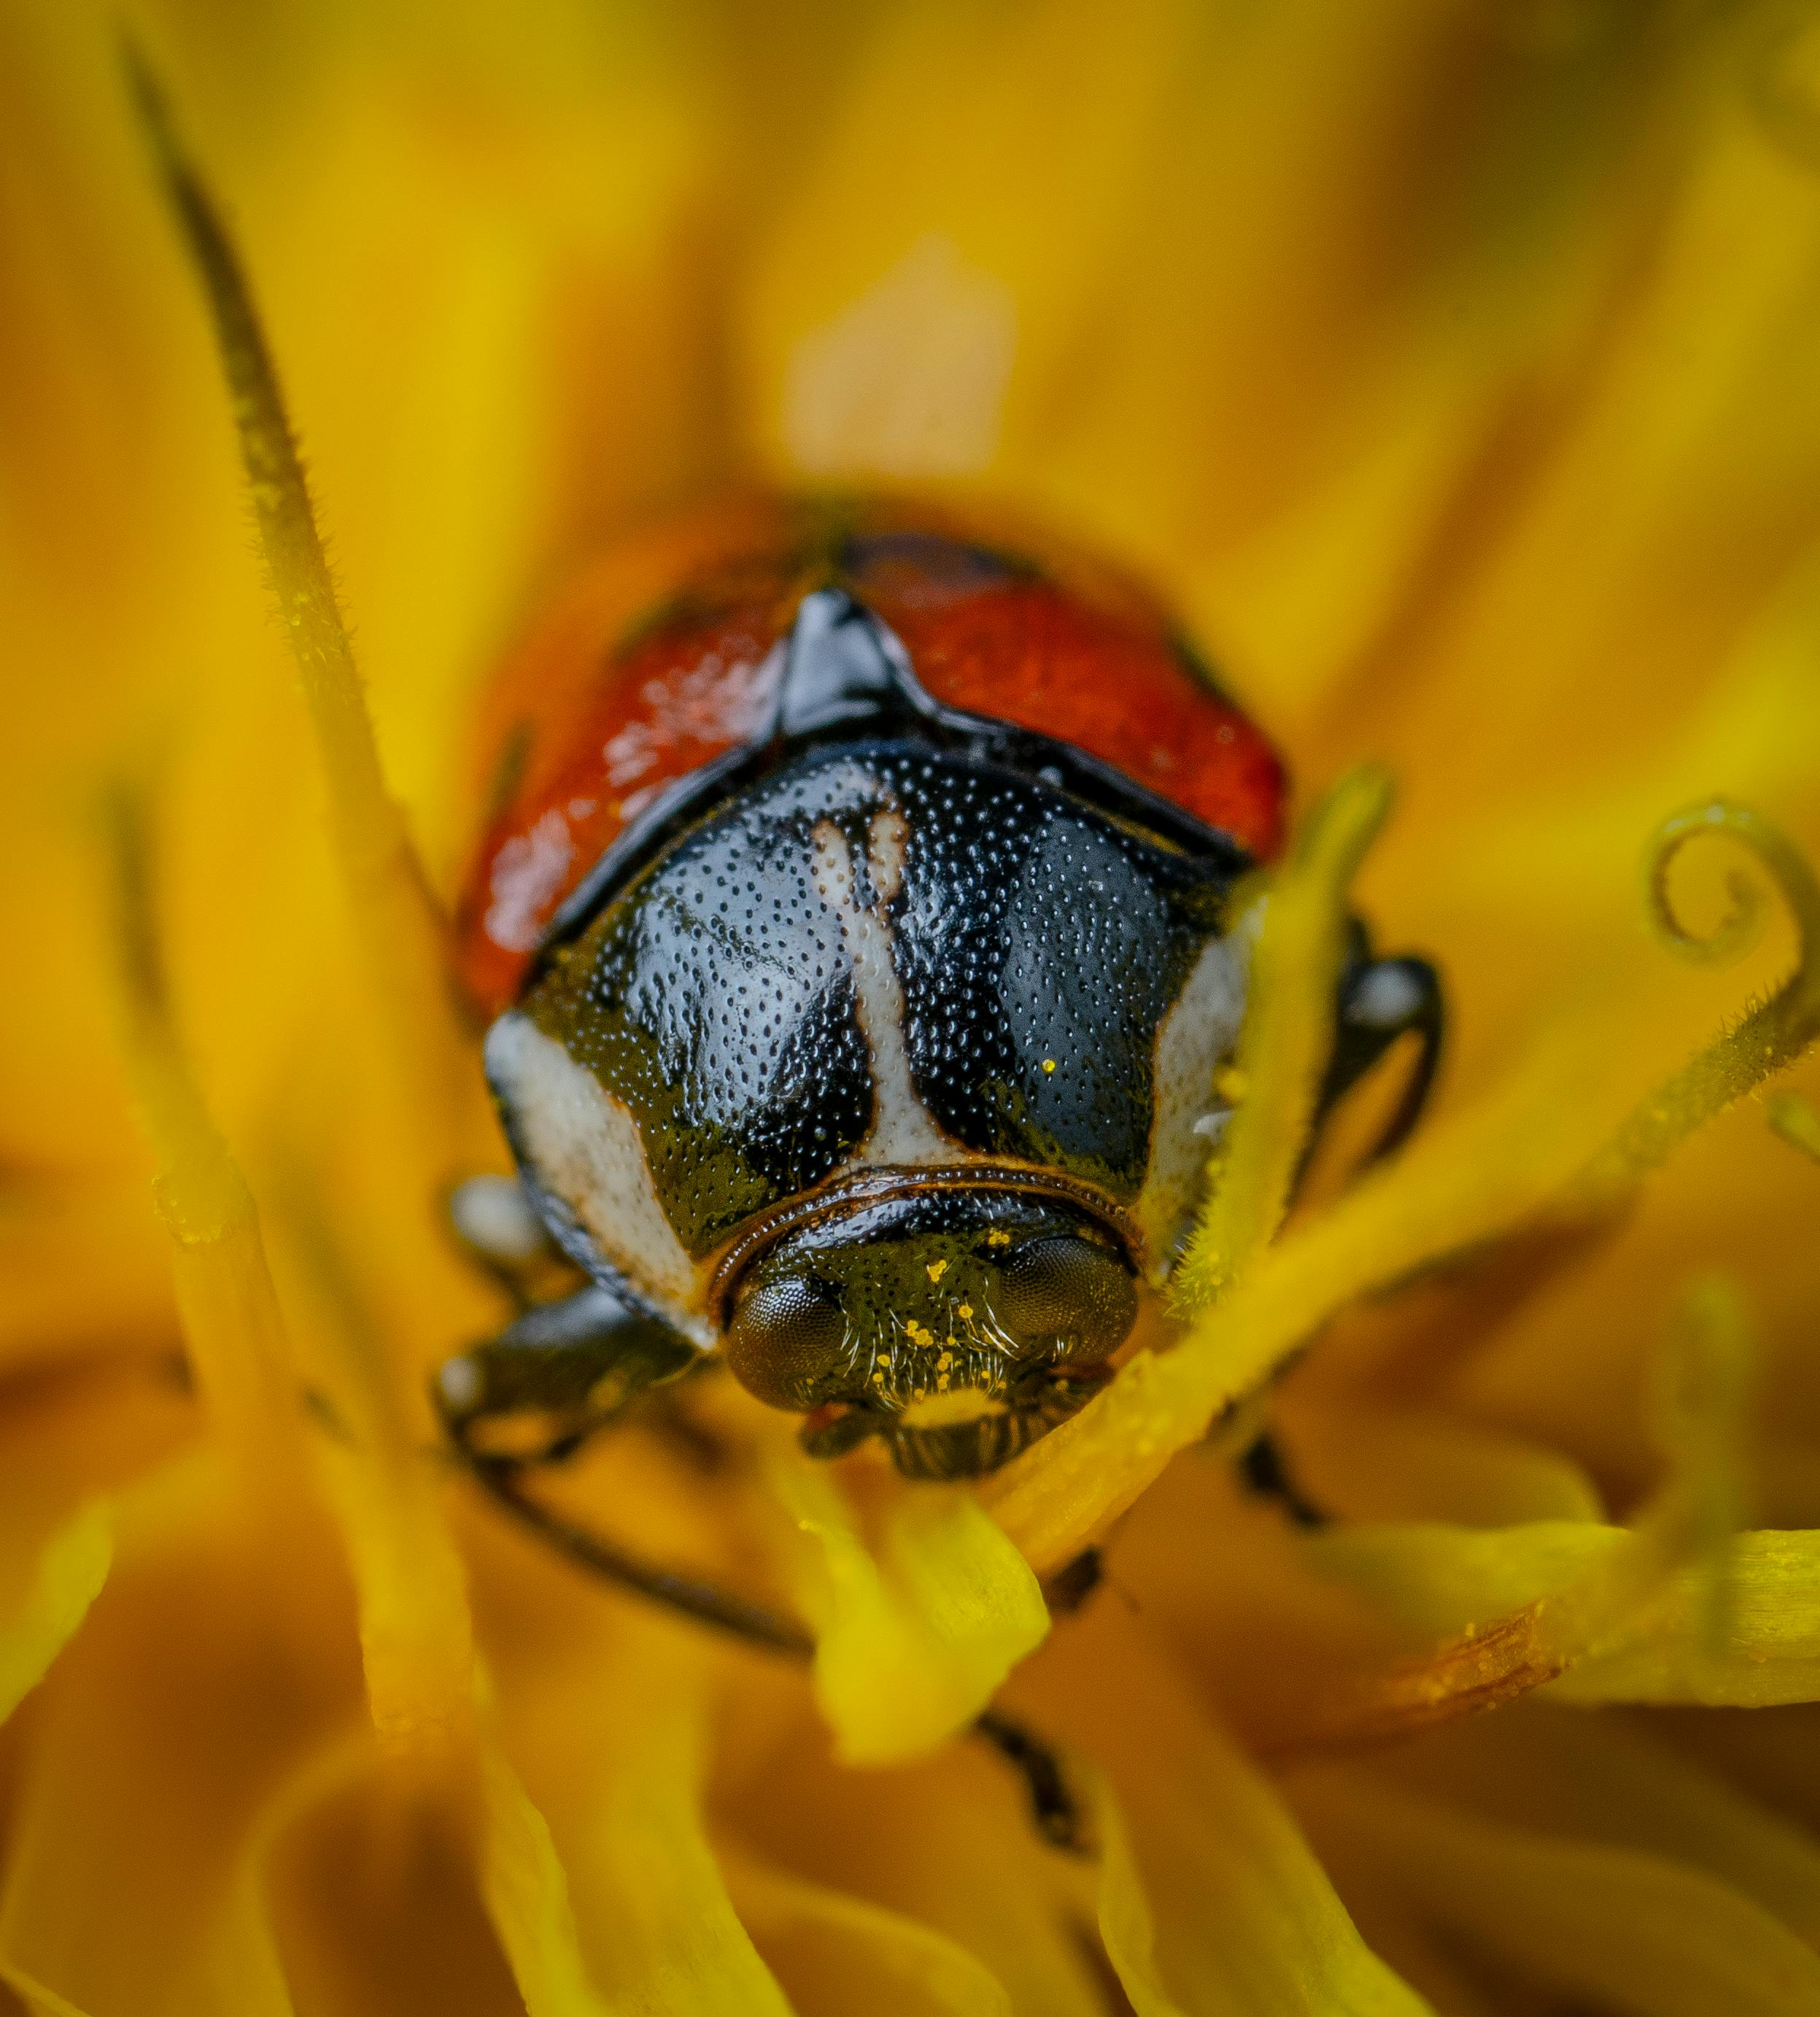
\includegraphics[width=0.8\textwidth]{sources/comparison/test_2.png}
  \caption{Resultados de compresión imagen 2}\label{fig:comparison2}
\end{figure}

\begin{figure}[htbp]
  \centering
  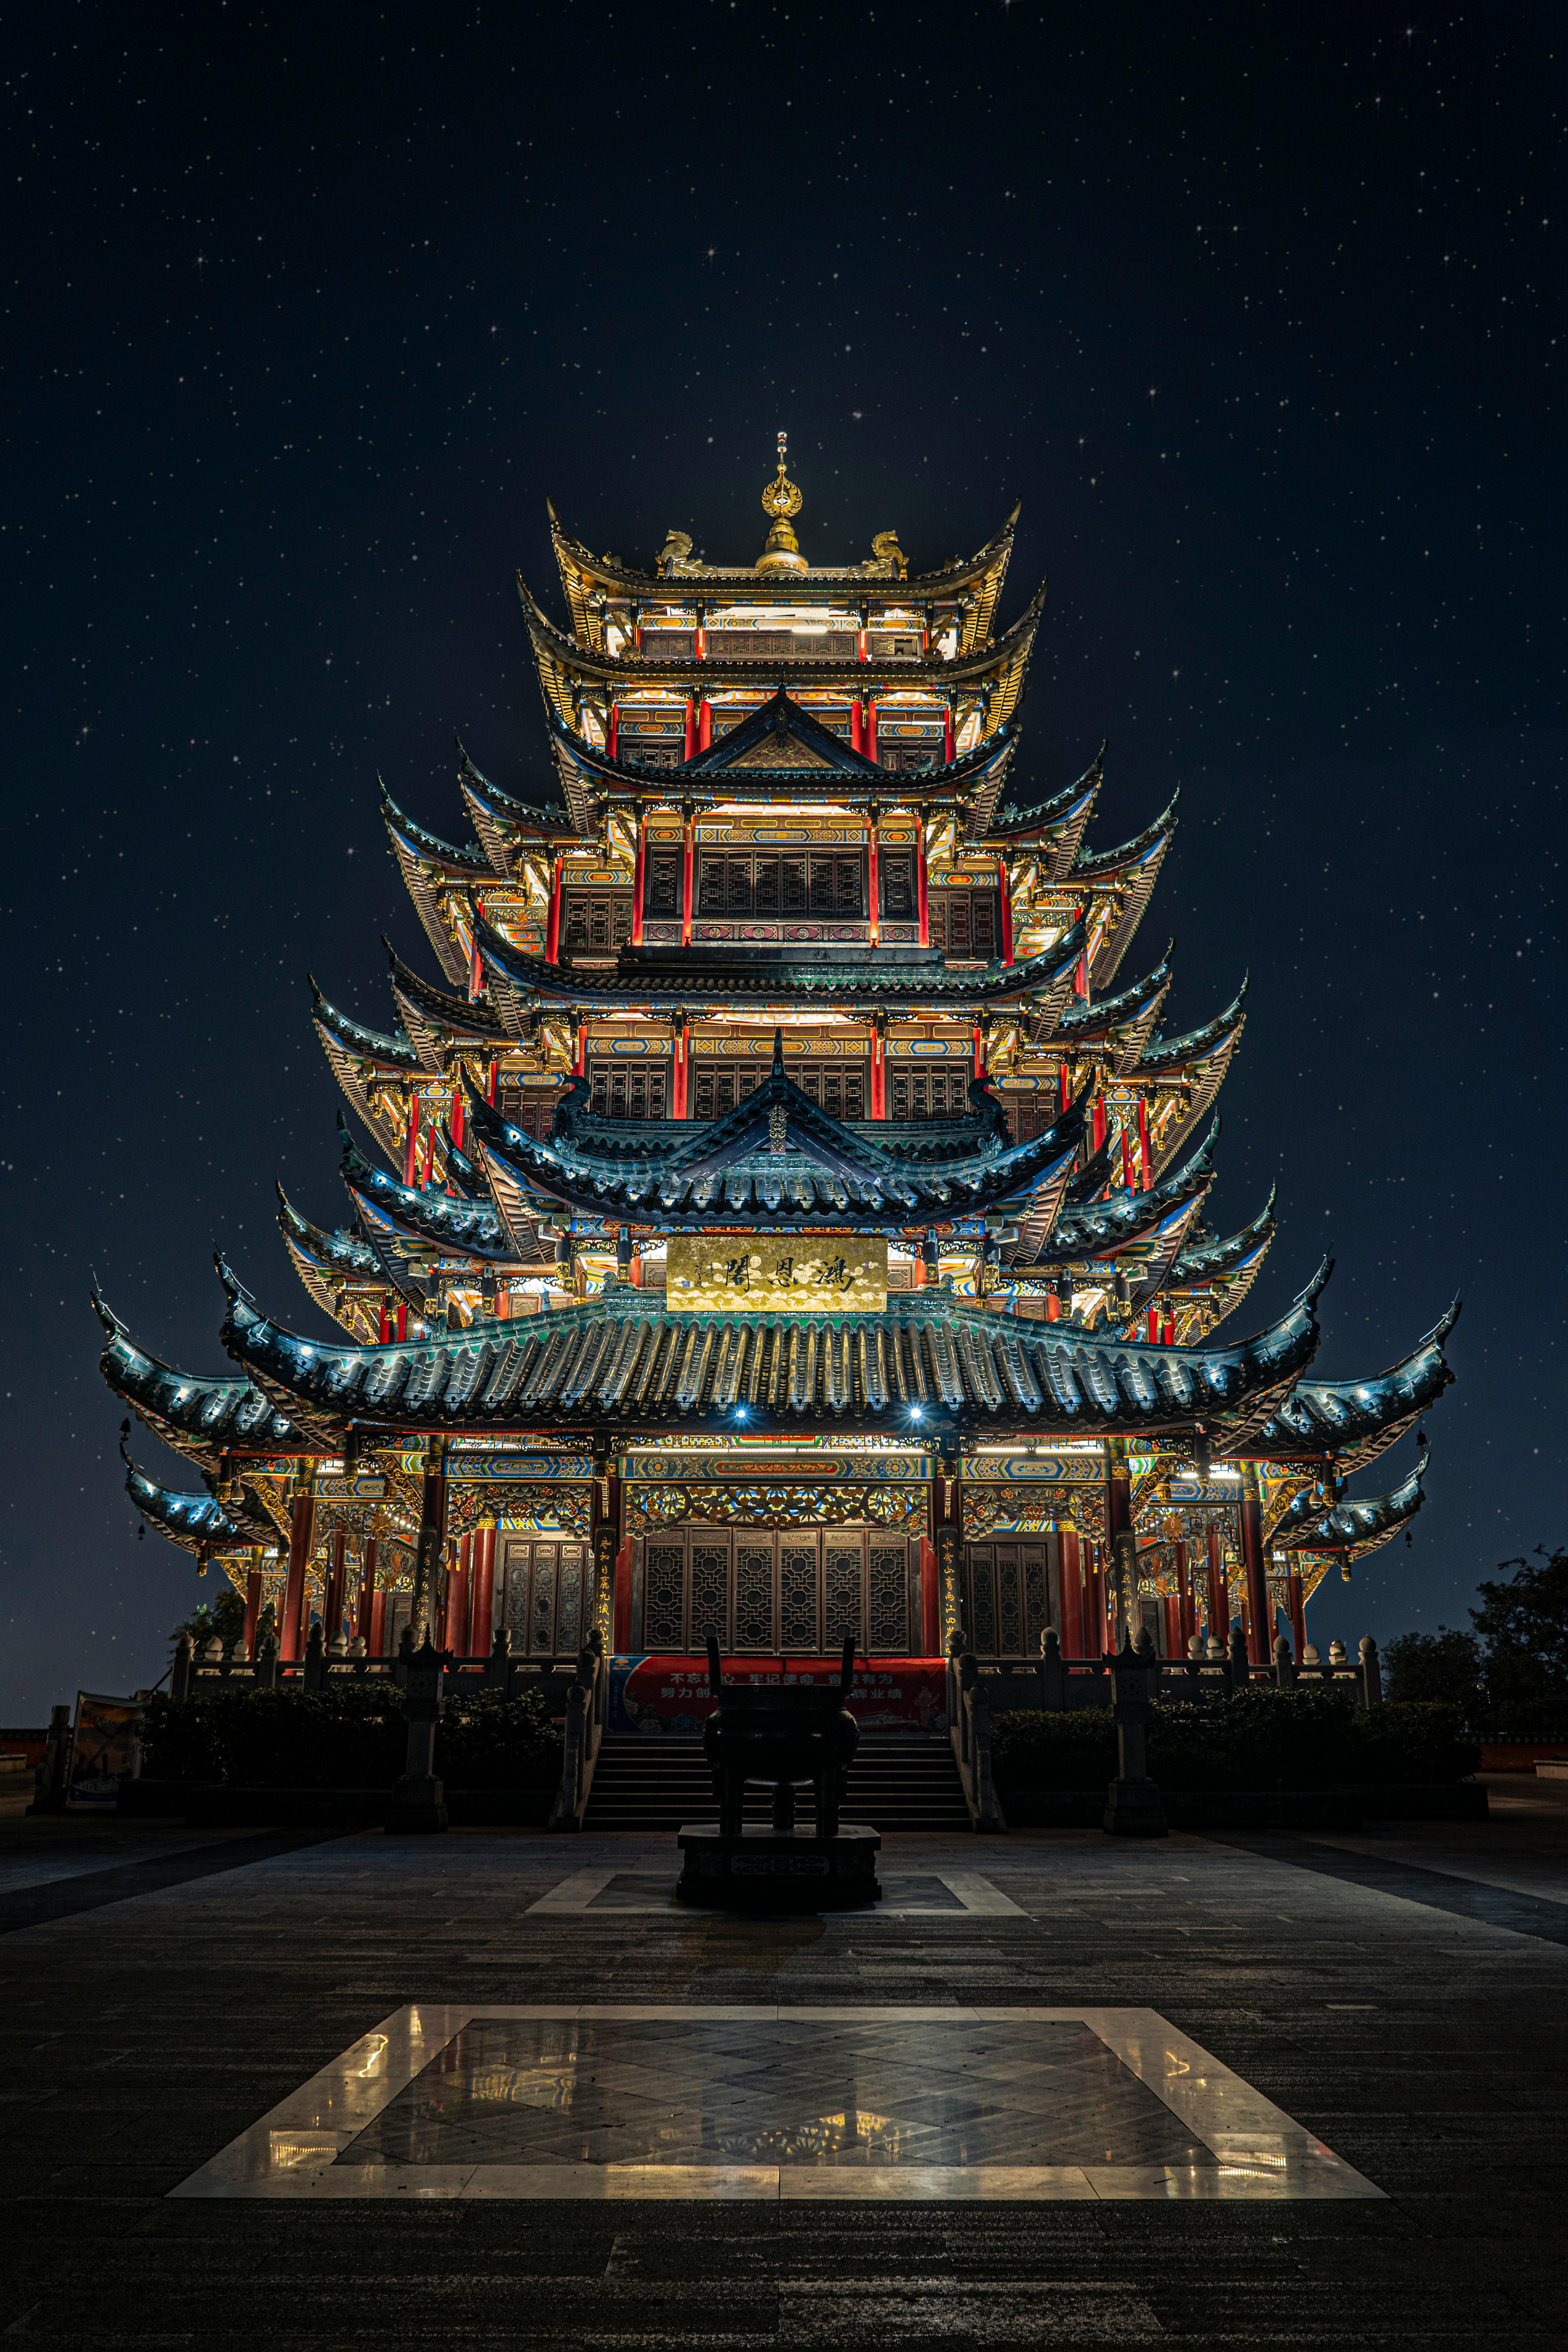
\includegraphics[width=0.8\textwidth]{sources/comparison/test_3.png}
  \caption{Resultados de compresión imagen 3}\label{fig:comparison3}
\end{figure}

\subsection{Observaciones sobre las imagenes}

Con la implementación del método basdado en FFT 2D se logro reducir el tamaño de los archivos sin sacrificar visualmente los detalles esenciales. Al transformar las imagenes se mantiene intacta una estructura general, contronos, gradaciones suaves y las texturas continuas.

Para las imagenes de color, el metodo FFT 2D logra reducir las imagenes entre un 50\% y un 60\% de su tamaño original. Esto se debe a que los 3 canales de color (rojo, verde y azul) comparten redundencias y el FFT 2D logra descartar muchas frecuencias sin que aparezca perceptibles.

Para las imágenes en escala de grises se puede observar que la compresión es menor, se logra reducir entre un 15\% y un 25\%, lo cual sigue siendo un tamaño considerable.

visualmente se puede observar que las imagenes son perfectamente perceptibles. Al ampliar la imagen comprimida, se puede percibir una ligera cantidad de ruido y algunos bordes ligeramente mas duros, pero cumple con la función de compresión.